\documentclass[10pt, a4paper]{article}
 
\usepackage{amsfonts, amsmath, amssymb}
\usepackage[utf8]{inputenc}
\usepackage[russian]{babel}
\usepackage[dvips]{graphicx}
\usepackage{listings}
 
\begin{document}

\begin{titlepage}
\newpage

\begin{center}
\vspace{1cm}
Московский государственный университет им. М.В. Ломоносова \\*
Факультет Вычислительной Математики и Кибернетики \\*
Кафедра Математических Методов Прогнозирования \\*
\end{center}


\vspace{8em}

\begin{center}
\Large Отчет к задаче:
\end{center}

\vspace{1.5em}

\begin{center}
\textsc{\textbf{``Восстановление плотности''}}
\end{center}

\vspace{6em}

\begin{flushright}
Кондрашкин Дмитрий Андреевич \\
\vspace{1.5em}
\end{flushright}

\vspace{\fill}

\begin{center}
2011
\end{center}

\end{titlepage}

\newpage
 
\section{Введение}
В общем виде задача восстановления плотности формулируется следующим образом\cite{voron}:

Задано множество объектов $X_m = \{x_1,\hdots,x_m\}$, выбранных случайно и независимо 
согласно неизвестному распределению $p(x)$. Требуется построить
эмпирическую оценку плотности -- функцию $\hat p(x)$, приближающую $p(x)$ на всём $X$.

В данной работе рассмотрены методы восстановления плотности:
\begin{itemize}
\item Параметрический
\item Непараметрический
\item Разделение смеси
\end{itemize}

В конце работы приведены примеры работы алгоритмов на реальных данных.

\newpage

\section{Восстановление плотности}
 
\subsection{Параметрический метод восстановления плотности}
В данной части работы будет исследован метод максимального правдоподобия для нормального распределения
(одно- и двумерный случаи).
Оценки максимального правдоподобия для нормального распределения:
$$
\hat \mu = \frac{1}{m}\sum_{i=1}^m x_i
$$
$$
\hat \sigma = \frac{1}{m-1}\sum_{i=1}^m \left(x_i-\hat \mu \right)\left(x_i-\hat \mu \right)^T
$$

Эксперимент проводился на идеальной выборке взятой из нормального распределения.
Генерация такой выборки проводилась с помощью функции normrnd в среде MATLAB.
Для оценки качества работы алгоритма были выбраны две метрики:
\begin{equation}
    \label{l2}
    \rho(f,g)=\frac{1}{m}\left(\sum_{i=1}^m\left(f(x_i)-g(x_i)\right)^2\right)^{\frac{1}{2}}
\end{equation}
\begin{equation}
    \label{cont}
    \rho(f,g)=\frac{1}{m}\sum_{i=1}^m\left|f(x_i)-g(x_i)\right|
\end{equation}
Формула~(\ref{l2}) представляет собой $l_2$ метрику, формула~(\ref{cont}) -- $l_1$ метрику, 
значения функций берутся в точках выборки, так как только в них нам надо оценивать плотность.

В ходе эксперимента были выявлены недостатки $l_1$ метрики. А именно было выявлено что это метрика не
адекватно оценивает качество работы алгоритма.
\nopagebreak[4]
\begin{figure}[h]
    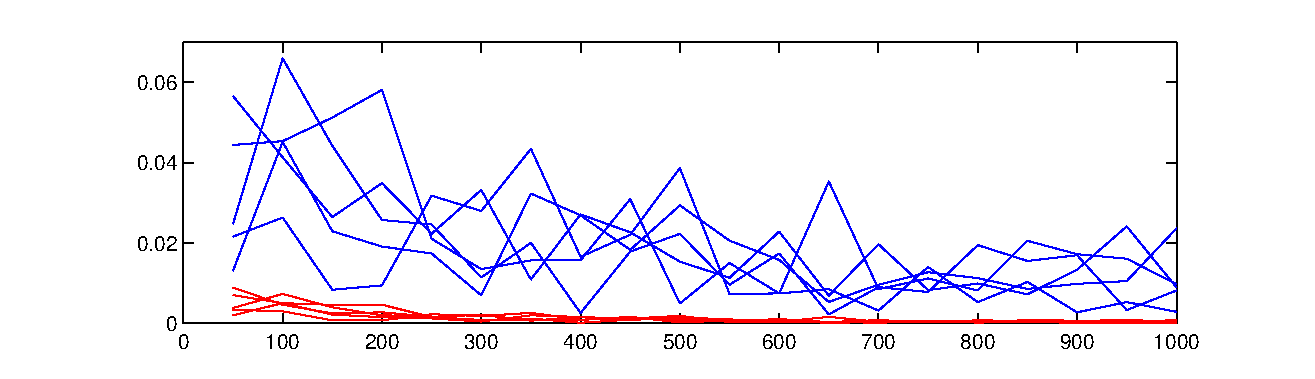
\includegraphics[width=\textwidth]{mle_quality.eps}
    \caption{Зависимость качества работы алгоритма от длины выборки}
    \label{mle_quality}
\end{figure}
\nopagebreak[4]

\nopagebreak[4]
На рис.~\ref{mle_quality} показана зависимость качества работы алгоритма от длины выборки.
Для каждого значения длины были проведены $5$ экспериментов, была посчитана $l_2$ и $l_1$
метрики. Заметим что значения $l_2$ метрики вытягиваются в одну линию при достаточно больших $N$
(точнее при $N\ge300$).
Графики равномерных метрик имеют резкие скачки, при этом не наблюдается какой-либо их зависимости от длины выборки.
Учитывая это, в дальнейшем для оценки качества алгоритмов восстановления плотности будем использовать только $l_2$ 
метрику.

На рис.~\ref{mle_quality_avg} представлено усреднение $l_2$ метрики по $100$ экспериментам.
\begin{figure}[h]
    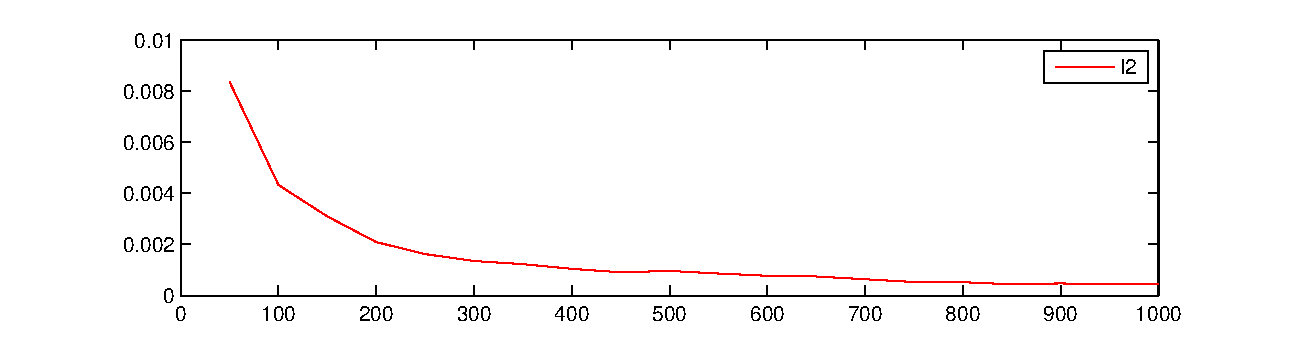
\includegraphics[width=\textwidth]{mle_quality_avg.eps}
    \caption{Усреднение $l_2$ метрики по $100$ экспериментам}
    \label{mle_quality_avg}
\end{figure}
Заметим что качество возрастает достаточно быстро, и уже при $N\ge300$ метод хорошо работает,
при дальнейшем увеличении $N$ улучшения несущественные.

Исследуем теперь работу метода при наличии шумов в выборке.
Пусть $X=(x_1, \hdots, x_n)$ -- идеальная выборка, взятая из $N(\mu,\sigma)$.
Добавим к ней выборку $Y=(y_1,\hdots,y_n)$ взятую из какого-либо другого распределения.
Полученную выборку $(X, Y)$ определим как зашумленную.

Установим максимальный размер внесенного шума, при котором метод максимального правдоподобия все еще дает
приемлемый результат. Для этого был проведен следующий эксперимент. В идеальную выборку длины $N=700$ из 
$N(2,1)$ вносился шум из $Exp(1)$. На рис.~\ref{noise_length} представлен график зависимости качества от 
размера внесенного шума. На рис.~\ref{noise_length_avg} та же самая зависимость после проведения усреднения 
по $100$ экспериментам.
\begin{figure}[h]
    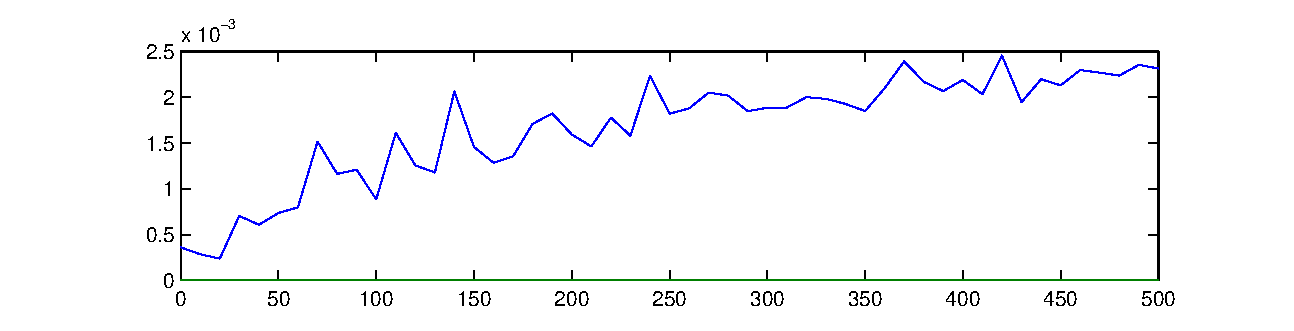
\includegraphics[width=\textwidth]{noise_length.eps}
    \caption{Зависимость качества от размера внесенного шума}
    \label{noise_length}
\end{figure}
\begin{figure}[h]
    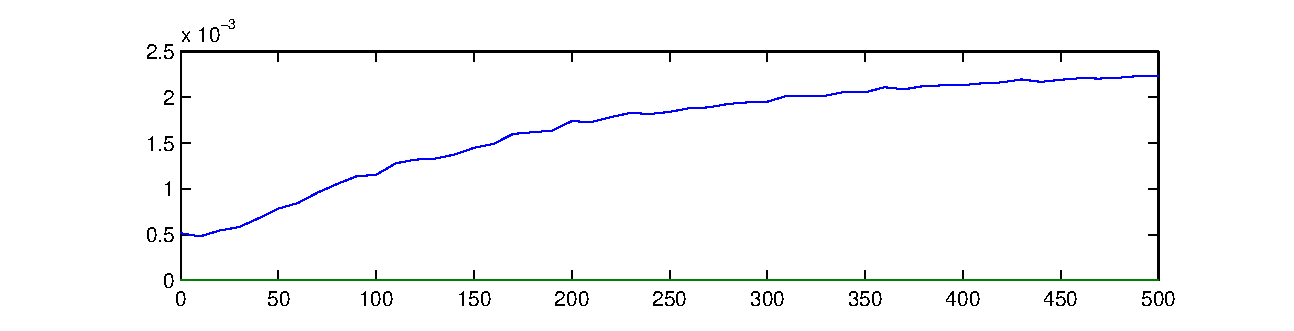
\includegraphics[width=\textwidth]{noise_length_avg.eps}
    \caption{Усреднение по 100 экспериментам}
    \label{noise_length_avg}
\end{figure}
Нетрудно заметить ухудшение качества при увеличении размера шума. Можно сказать что при размере шума
$M\le50$ качество остается на приемлемом уровне. Далее идет достаточно резкое ухудшение.
При $M\ge200$ по всей видимости метод перестает выдавать что-либо адекватное.

На рис.~\ref{ideal_nle} приведен пример работы алгоритма на идеальной выборке.
\begin{figure}[h]
    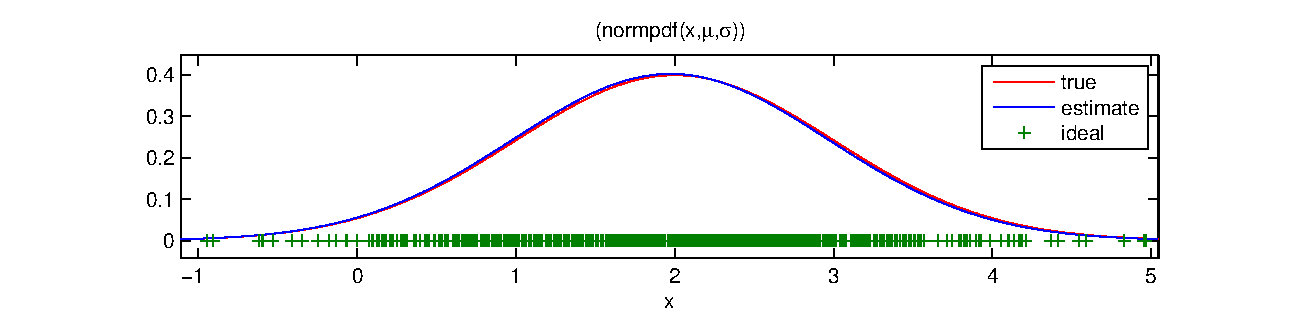
\includegraphics[width=\textwidth]{ideal_nle.eps}
    \caption{Идеальная выборка}
    \label{ideal_nle}
\end{figure}

На рис.~\ref{middle_noised_nle} и рис.~\ref{heavy_noised_nle} приведен пример работы на зашумленных выборках.
\begin{figure}[h]
    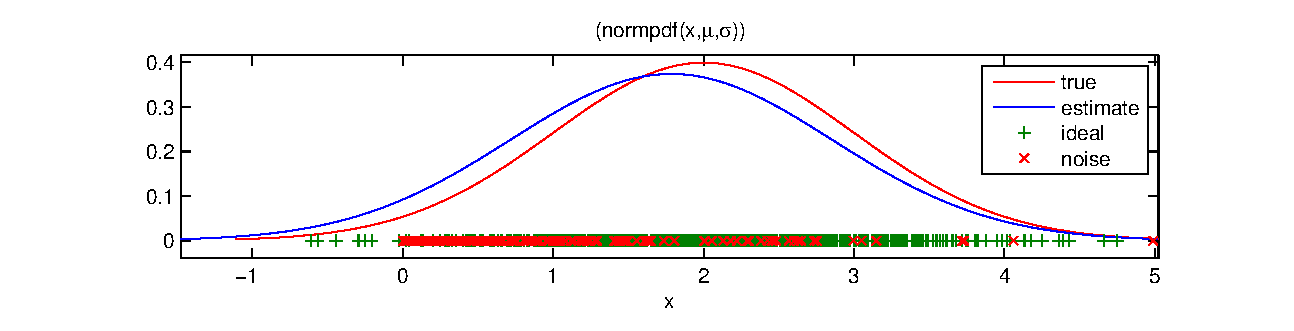
\includegraphics[width=\textwidth]{middle_noised_nle.eps}
    \caption{Выборка со средним зашумлением}
    \label{middle_noised_nle}
\end{figure}
\begin{figure}[h]
    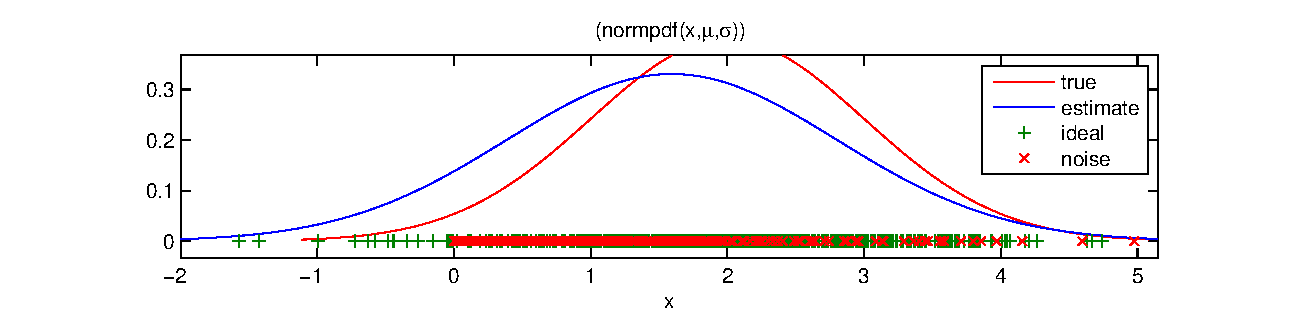
\includegraphics[width=\textwidth]{heavy_noised_nle.eps}
    \caption{Сильно зашумленная выборка}
    \label{heavy_noised_nle}
\end{figure}

На рис.~\ref{parametric_2est} приведен график восстановленной плотности -- результат работы алгоритма в двумерном случае.
На рис.~\ref{parametric_2l2} приведен график $l_2$ метрики -- оценка качества.
Оцениваемое распределение имело параметры:
\begin{equation}
\mu=\left(\begin{matrix}
    1 && -1
\end{matrix}\right)
\label{mu}
\end{equation}
\begin{equation}
\Sigma=\left(\begin{matrix}
    0.9 && 0.4 \\
    0.4 && 0.3
\end{matrix}\right)
\label{sigma}
\end{equation}

\begin{figure}[t]
    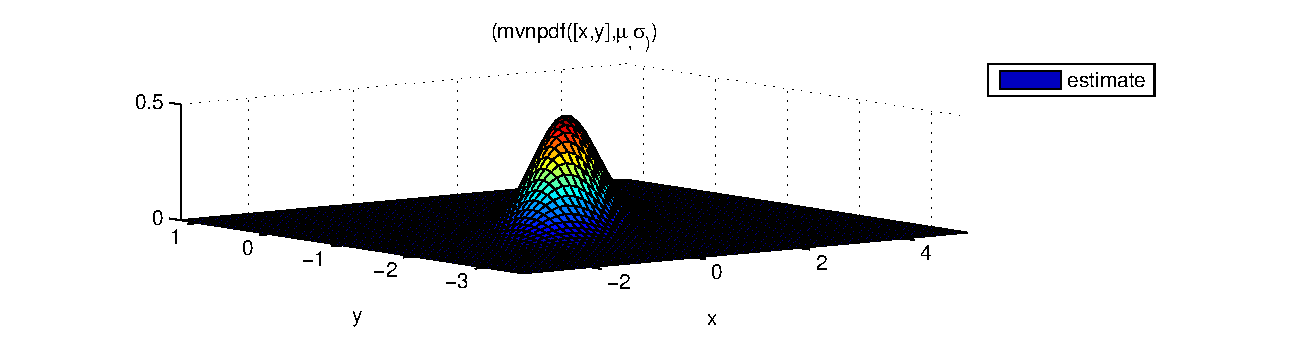
\includegraphics[width=\textwidth]{parametric_2est.eps}
    \caption{Двумерный ММП}
    \label{parametric_2est}
\end{figure}
\begin{figure}[t]
    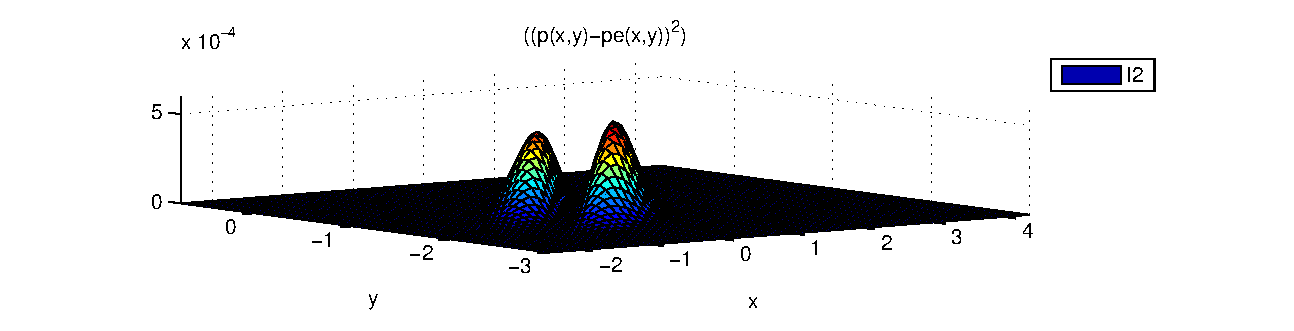
\includegraphics[width=\textwidth]{parametric2_l2.eps}
    \caption{$l_2$ метрика -- оценка качества}
    \label{parametric_2l2}
\end{figure}

\clearpage

\subsection{Непараметрический метод восстановления плотности}
Непараметрический метод восстановления плотности будет исследован на примере алгоритма Парзеновского окна.
Парзеновская оценка плотности записывается следующим образом:
$$
\frac{1}{mh}\sum_{i=1}^m K\left(\frac{x-x_i}{h}\right)
$$
где $h$ -- ширина окна, $m$ -- длина выборки, $K(x)$ -- функция ядра.

Наиболее популярныe ядра представлены в таблице~\ref{kernels}.

\begin{table}[h]
    \begin{tabular}{|l|l|}
        \hline
        \text{Епанечникова} & $E(r)=\frac{3}{4}(1-r^2)[|r|\le1]$\\
        \hline
        \text{Квартичесоке} & $Q(r)=\frac{15}{16}(1-r^2)^2[|r|\le1]$\\
        \hline
        \text{Треугольное} & $T(r)=(1-|r|)[|r|\le1]$\\
        \hline
        \text{Гауссовское} & $G(r)=(2\pi)^{-\frac{1}{2}}e^{-\frac{1}{2}r^2}$\\
        \hline
        \text{Прямоугольное} & $\Pi(r)=\frac{1}{2}[|r|\le1]$\\
        \hline
    \end{tabular}
    \caption{Примеры функций ядра}
    \label{kernels}
\end{table}

Подробнее об этом методе можно прочитать в~\cite[\S~2.2]{voron}.

Исследуем зависимость качества алгоритма от ширины окна.
Для нормального распределения известна оценка:
\begin{equation}
    h=\left(\frac{4\hat \sigma^5}{3n}\right)^{\frac{1}{5}}\approx 1.06\hat \sigma n^{-\frac{1}{5}}
    \label{opt_h}
\end{equation}
где $\hat \sigma$ стандартное отклонение.

\begin{figure}[h]
    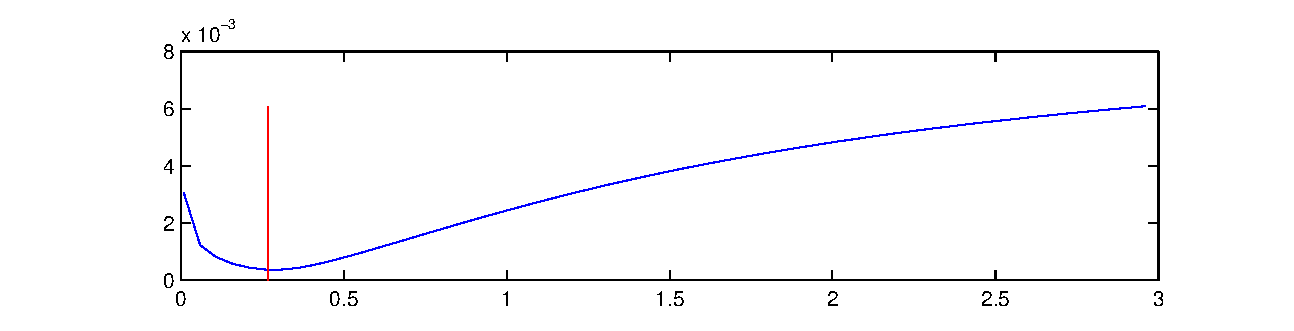
\includegraphics[width=\textwidth]{h_eval.eps}
    \caption{Зависимость качества от ширины окна, $N(0,1)$}
    \label{h_eval}
\end{figure}
\begin{figure}[h]
    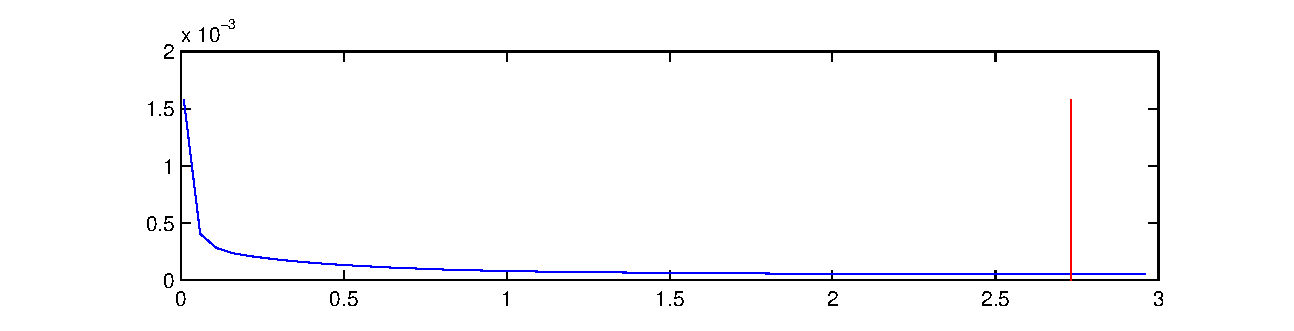
\includegraphics[width=\textwidth]{h_sigma10.eps}
    \caption{Зависимость качества от ширины окна, $N(0,10)$}
    \label{h_sigma10}
\end{figure}

На рис.~\ref{h_eval} показана зависимость $l_2$ метрики качества от ширины окна $h$. Эксперимент проводился на
выборке длиной $N=1000$ из $N(0,1)$. Красной линией отмечено значение полученное с помощью оценки~(\ref{opt_h}).
Еще один подобный график приведен на рис.~\ref{h_sigma10}, но здесь уже выборка взята из $N(0,10)$.

Можно сделать следующий вывод: ширина окна зависит от выборки, например от дисперсии.

Представленная теоретическая оценка ширины окна~(\ref{opt_h}) оказалась достаточно эффективной, поэтому в дальнейших
экспериментах будем ее использовать.

Был проведен эксперимент для выявления зависимости качества от функции ядра.
Алгоритм запускался 5 раз на выборке из $N(0,1)$ длиной $N=1000$ для каждой функции ядра. 
Результаты(значения $l_2$ метрики) приведены в таблице~\ref{kernel_eval}.

\begin{table}[h]
    \begin{tabular}{|l|l|l|l|l|l|l|l|}
        \hline
        Ядро&1&2&3&4&5&Среднее\\
        \hline
        E&0.55492&0.75366&0.63257&0.95485&0.87299&0.37690\\
        \hline
        K&0.64844&0.80081&0.64817&1.10600&0.95006&0.41535\\
        \hline
        T&0.61527&0.77803&0.63657&1.04280&0.91577&0.39884\\
        \hline
        G&0.25949&0.58484&0.71670&0.31783&0.67155&0.25504\\
        \hline
        P&0.45575&0.71871&0.66278&0.74646&0.77969&0.33634\\
        \hline
    \end{tabular}
    \caption{Зависимость качества от ядра($\times 10^{-3}$)}
    \label{kernel_eval}
\end{table}

Неудивительно что Гауссовское ядро показало лучший результат, мы ведь оценивали нормальное распределение!
Между остальными ядрами разницы практически нет.

На рис.~\ref{parzen1_500},~\ref{parzen1_2000} приведены примеры работы алгоритма при разных длинах выборки.
\begin{figure}[h]
    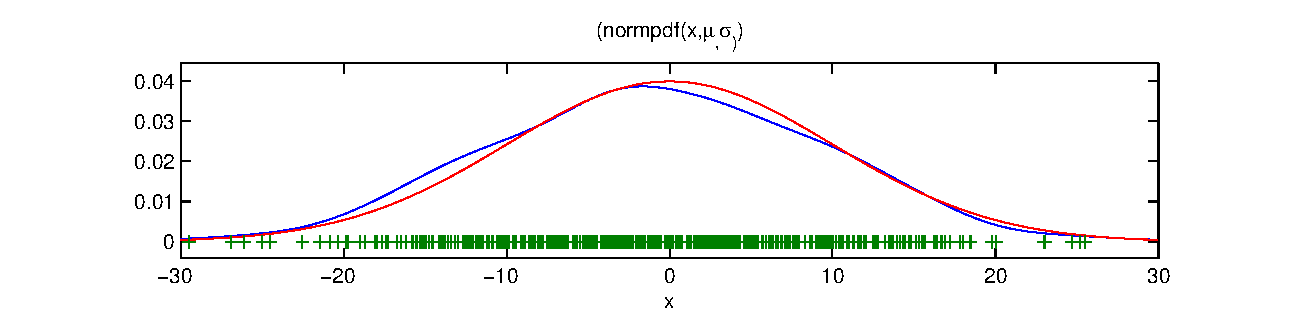
\includegraphics[width=\textwidth]{parzen1_500.eps}
    \caption{$N=500$}
    \label{parzen1_500}
\end{figure}
\begin{figure}[h]
    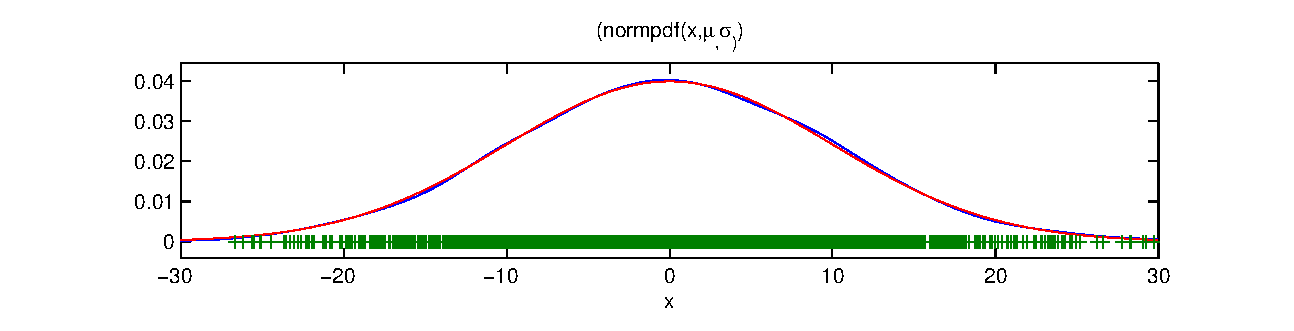
\includegraphics[width=\textwidth]{parzen1_2000.eps}
    \caption{$N=2000$}
    \label{parzen1_2000}
\end{figure}

На рис.~\ref{parzen2} приведен пример работы двумерного алгоритма на выборке длиной $N=2000$ из 
двумерного нормального распределения с параметрами~(\ref{mu}), (\ref{sigma}). Ошибка (в $l_2$ смысле)
составила $6.9\times 10^{-4}$.
\begin{figure}[h]
    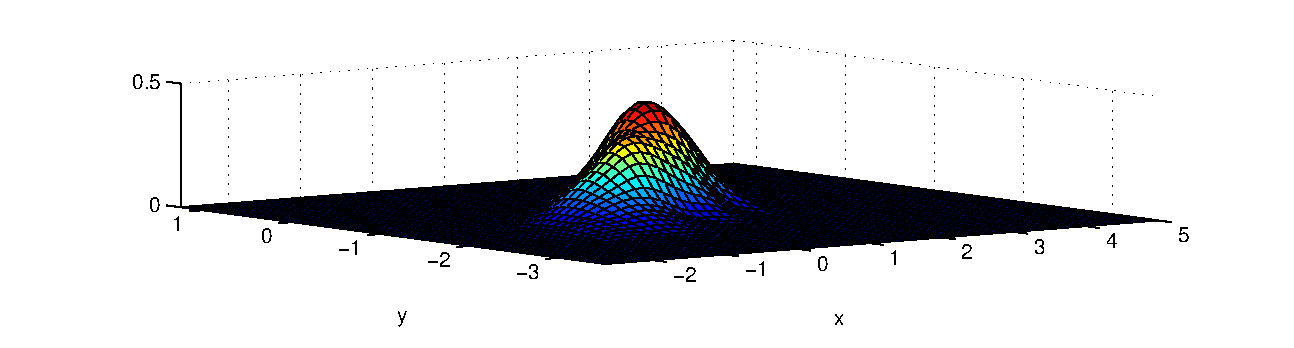
\includegraphics[width=\textwidth]{parzen2.eps}
    \caption{Двумерная модификация}
    \label{parzen2}
\end{figure}

\newpage

\subsection{EM-алгоритм}
В этой части работы рассмотрено исследование EM-алгоритма. Подробное описание алгоритма 
можно посмотреть в~\cite[\S~2.4]{voron}.

Алгоритм принимает на вход три параметра $(X,k,\delta)$ где $X$--выборка, $k$--количество компонент,
$\delta$--параметр критерия останова.

В качестве начального приближения для весов $w$ брались значения $\frac{1}{k}$, для векторов $\mu_j$:
$$
\mu_j=min(X)+\frac{j-1}{k}(max(X)-min(X))+\zeta
$$
где $\zeta$ -- некая случайная величина. Для $\Sigma_j$ брались единичные матрицы.

Был также реализован стохастический EM-алгоритм. Было проведено сравнение классического и стохастического вариантов.
Алгоритмы тестировались на смесях из нормальных распределений со следующими параметрами:
$$
w=\left(\begin{matrix}
    \frac{1}{3} & \frac{2}{3}
\end{matrix}\right)
$$
$$
\mu=\left(\begin{matrix}
    1 & 5
\end{matrix}\right)
$$
$$
\sigma=\left(\begin{matrix}
    1&1
\end{matrix}\right)
$$
Было проведено 5 экспериментов с $\delta=0.01$. Результаты приведены в
 таблицах~\ref{time},~\ref{rate},~\ref{iter}.

\begin{table}[h]
    \begin{tabular}{|l|l|l|l|l|l|}
        \hline
        &1&2&3&4&5\\
        \hline
        EM&7.2331&5.5446&7.1165&8.3881&7.6706\\
        \hline
        SEM&4.2709&4.2506&7.0584&5.4981&2.5923\\
        \hline
    \end{tabular}
    \caption{Время работы алгоритма (процессор Core2Duo @ 1,86GHz)}
    \label{time}
\end{table}

\begin{table}[h]
    \begin{tabular}{|l|l|l|l|l|l|}
        \hline
        &1&2&3&4&5\\
        \hline
        EM&0.65698&0.31528&0.49616&0.33791&0.19582\\
        \hline
        SEM&0.15251&0.19378&0.26555&0.18751&0.40061\\
        \hline
    \end{tabular}
    \caption{Качество($l_2$) работы алгоритма($\times 10^{-3}$)}
    \label{rate}
\end{table}

\begin{table}[h]
    \begin{tabular}{|l|l|l|l|l|l|}
        \hline
        &1&2&3&4&5\\
        \hline
        EM&9&7&9&11&10\\
        \hline
        SEM&14&14&23&18&9\\
        \hline
    \end{tabular}
    \caption{Количество итераций}
    \label{iter}
\end{table}

Стохастический ЕМ-алгоритм работает быстрее и качественнее, его работа меньше зависит от начального
приближения

На рис.~\ref{EM1} приведен пример работы ЕМ-алгоритма, на рис.~\ref{SEM1} -- стохастического ЕМ-алгоритма.
\begin{figure}[h]
    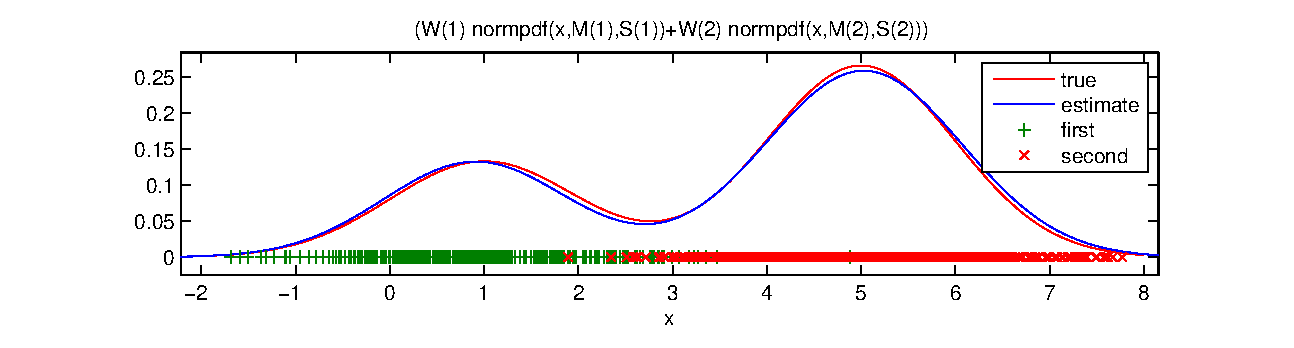
\includegraphics[width=\textwidth]{EM1.eps}
    \caption{Пример работы ЕМ-алгоритма}
    \label{EM1}
\end{figure}
\begin{figure}[h]
    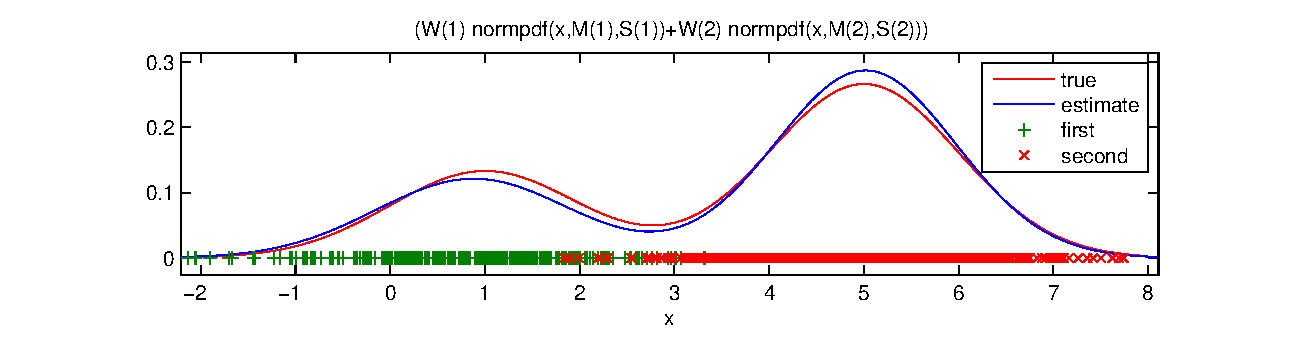
\includegraphics[width=\textwidth]{SEM1.eps}
    \caption{Пример работы стохастического ЕМ-алгоритма}
    \label{SEM1}
\end{figure}

\clearpage
\section{Эксперимент на реальных данных}
Эксперимент был проведен на серии реальных данных. Данные содержат информацию о 272 извержениях гейзера Old Faithful,
каждое из которых характеризуется длительностью извержения и временем до следующего извержения.  
На рис.~\ref{data} показаны исходные данные.
Результат работы ЕМ-алгоритма показан на рис.~\ref{EMans},~\ref{EMansXY}.
\begin{figure}[h]
    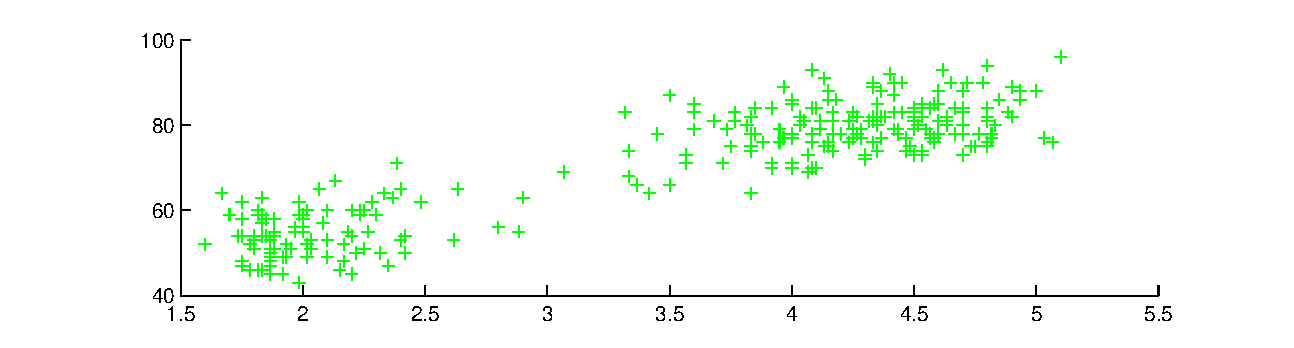
\includegraphics[width=\textwidth]{data.eps}
    \caption{Данные об извержениях}
    \label{data}
\end{figure}
\begin{figure}[h]
    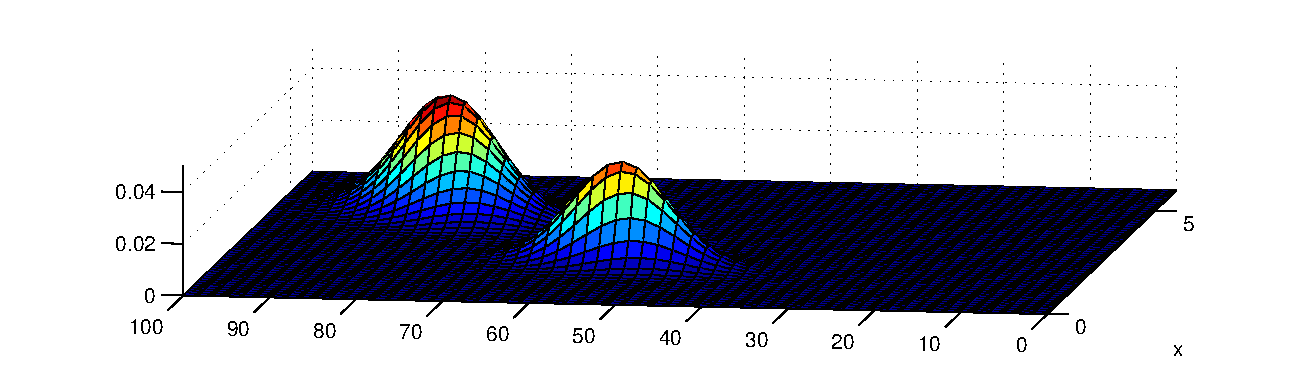
\includegraphics[width=\textwidth]{EMans.eps}
    \caption{Плотность(EM)}
    \label{EMans}
\end{figure}
\begin{figure}[h]
    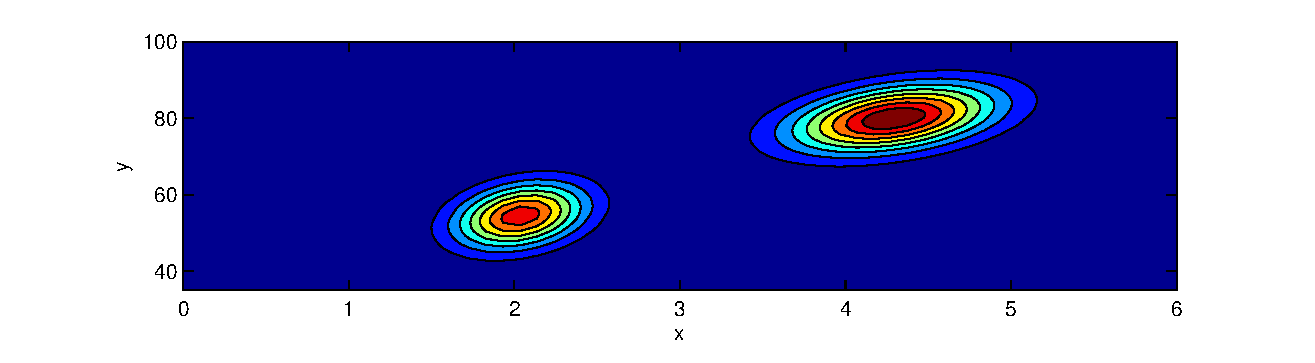
\includegraphics[width=\textwidth]{EMansXY.eps}
    \caption{Плотность(EM), XY проекция, линии уровня}
    \label{EMansXY}
\end{figure}

Так же была предпринята попытка решения этой задачи с помощью метода Парзеновского окна.
В ходе нескольких экспериментов была подобрана ширина окна: по оси $X$ -- $h=1$, по оси $Y$ -- $h=2$.
На рис.~\ref{ParzenAns},~\ref{ParzenAnsXY} можно увидеть результат.

Данный результат несомненно можно улучшить, например более аккуратно подбирая ширину окна(здесь 
можно использовать кросс-валидацию).
\begin{figure}[h]
    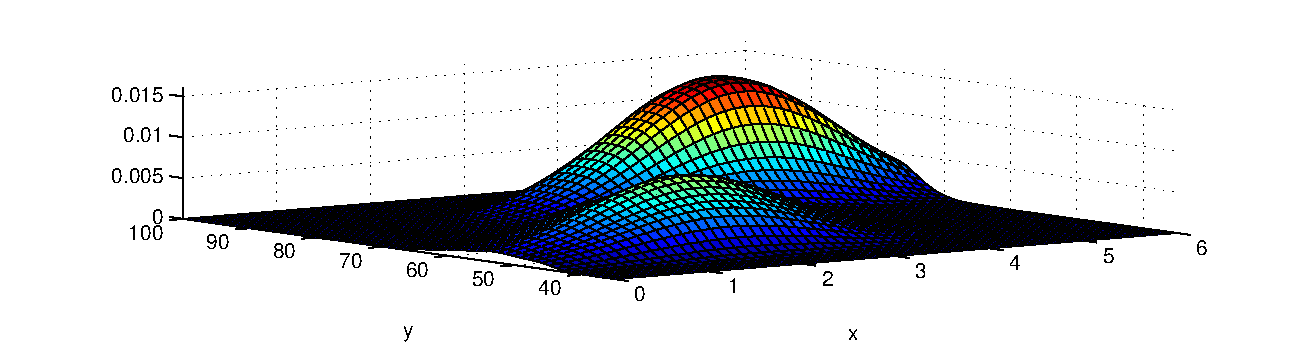
\includegraphics[width=\textwidth]{parzenAns.eps}
    \caption{Плотность(Парзеновское окно)}
    \label{ParzenAns}
\end{figure}
\begin{figure}[h]
    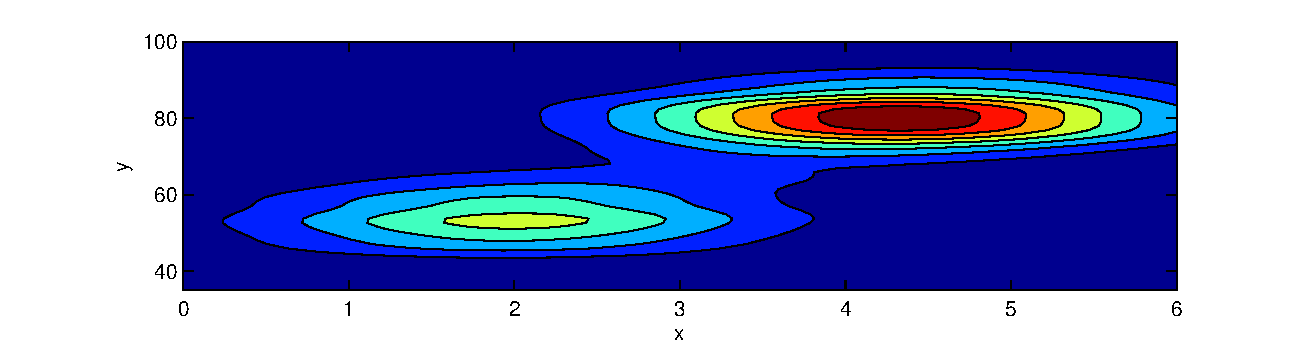
\includegraphics[width=\textwidth]{parzenAnsXY.eps}
    \caption{Плотность(Парзеновское окно), XY проекция, линии уровня}
    \label{ParzenAnsXY}
\end{figure}


\clearpage
\begin{thebibliography}{99}
    \bibitem{voron}Воронцов К. В. Машинное обучение, Курс лекций.
    \bibitem{dj}Дьяконов A. Г. Анализ данных, обучение по прецедентам, логические игры, системы WEKA, RapidMiner и MatLab.
\end{thebibliography}

\end{document}
